\chapter{Structures de donn�es}
\label{chapitre_structures}

L'utilisation de structures de donn�es adapt�es aux proc�dures d'optimi\-sation est un �l�ment cl� du processus de conception. Un des principes cl�s r�side dans l'utilisation de tableaux � acc�s direct indic�s par identifiant.

Nous donnons ci-dessous, une description des �l�ments cl�s de la mod�li\-sation orient�e objet sous forme de diagramme UML. Sont pr�sent�s, les composants de base, les tableaux de donn�es, l'environnement commun d'optimisation.

\section{Structure position}

%\setlength\abovecaptionskip{0cm}

\begin{figure}[h]
 \begin{center}
  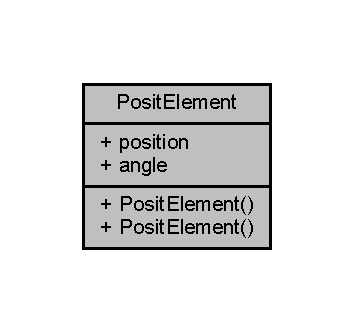
\includegraphics[scale=1]{./Img/struct_posit_element__coll__graph.pdf}
  \caption {Position d'un �l�ment/composant.}
  \label{uml:position}
 \end{center}
\end{figure}

Tout composant g�om�trique est caract�ris� par un point de r�f�rence et un angle d'orientation. Sa position dans le plan est d�termin�e par la position du point de r�f�rence dans le plan et l'angle avec l'horizontale. Le diagramme de classe UML est donn� par la figure \ref{uml:position}.

\section{Objet solution}

\begin{figure}[h]
 \begin{center}
  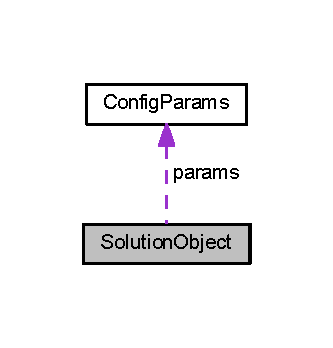
\includegraphics[width=\columnwidth]{./Img/class_solution_object__coll__graph.pdf}
  \caption {Classe principale solution.}
  \label{uml:solution}
 \end{center}
\end{figure}

La classe \textit{SolutionObject} est la structure principale repr�sentant une solution du probl�me. Elle comporte toutes les variables de la solution, variables de positionnement, d'ordonnancement. Chaque solution manipul�e et/ou construite par l'algorithme d'optimisation est une instance de la classe \textit{SolutionObject}. Une solution peut �tre dupliqu�e et reproduite � volont� � l'aide de l'op�rateur d'affectation standard (=). La solution est un objet manipul� par les algorithmes m�taheuristiques de r�solution. Le diagramme de classe UML est donn� par la figure \ref{uml:solution}. Seule la classe de configuration \textit{ConfigParams} apparait ici.


